\section{AND\=aNA-v2 Design} \label{sec:design}
In this section we describe the much improved design of {\sf AND\=aNAv2}. Table \ref{tab:notation} introduces the relevant notation needed to understand the design in its entirety. 

\begin{table*}
\centering
\caption{Notation used in the presentation of this work.}
\label{tab:notation}
  \begin{tabular}{| r | l |} \hline
  $\mathsf{C}$ & Set of all consumers  \\
  $\mathsf{P}$ & Set of all producers  \\ 
  $\mathsf{R}$ & Set of all routers  \\
  $\mathsf{IF}$ & Set of all interfaces on all routers  \\
  $\mathsf{if}_i^r \in \mathsf{IF}$ & Interface $i$ of router $r$  \\
  $(pk_i, sk_i)$ & Public/private key pair for router $r$  \\
  $\overline{\mathsf{int}}_{i}^{j}$ & Encrypted interest wrapped from router $i$ to router $j$ ($i \leq j$)  \\
  $\mathcal{A}$ & Adversary \\ 
  $u$ & Entity in the network (consumer or producer) \\
  $u \to_{\mathsf{int}} r$ & Entity $u$ sends interest to router $r$  \\ 
  $\mathsf{int} \to \mathsf{if}_i^r$ & Interest $\mathsf{int}$ is sent to interface $i$ of router $r$ \\
  $r \in \mathsf{R}$ & An anonymizing router (AR) \\ 
  $\mathcal{E}_{pk_i}(\cdot)$ & Public key encryption using $pk_i$ \\ 
  $\mathcal{D}_{pk_i}(\cdot)$ & Public key decryption using $pk_i$ \\ 
  $\mathsf{Encrypt}_{k_i}(\cdot)$ & Symmetric key encryption using key $k_i$ \\ 
  $\mathsf{Decrypt}_{k_i}(\cdot)$ & Symmetric key decrypt using key $k_i$ \\ 
  $\mathsf{ST}$ & AR session table used to store session ID and digest tuples \\
  $H$ & A collision resistant hash function on the domain $\{0,1\}^*$ to range $\{0,1\}^{\kappa}$ \\
  $F_k$ & A keyed pseudorandom function \\ \hline
  \end{tabular}
\end{table*}

\subsection{Circuit and Session Establishment}
At the heart of the {\sf AND\=aNAv2} is the notion of anonymizing routers and connection-oriented circuits, similar in spirit to the inner workings of TOR \cite{Tor}. Anonymizing routers serve two purposes in {\sf AND\=aNAv2}: (1) to decapsulate and forward encrypted interests, along with content encryption keys, generated by a consumer until the cleartext interest arrives at the producer, and (2) to encapsulate sensitive content using the previously acquired encryption keys and relay the encrypted content downstream. In this way, the consumer generates an interest wrapped by several layers of encryption and receives a piece of content wrapped in several layers of encryption that it can easily decrypt. It is also important to note that since each anonymizing router operates at the application layer, it effectively serves as the producer for each downstream router in the {\sf AND\=aNAv2} circuit. Therefore, NDN policy dictates that such content \emph{must be signed}. Verification of content from upstream routers, however, is not mandatory. 

We also note that the current {\sf AND\=aNAv2} design has support for two types of circuits: asymmetric and symmetric session-based. In the asymmetric variant, all encrypted interests are done using a CCA-secure PKI scheme and all content is encrypted using a CCA-secure symmetric key encryption scheme. Conversely, in the session-based variant, all encrypted interests are protected using a CCA-secure symmetric key encryption scheme, where the key is identified using a unique session identifier sent in the cleartext along with the encrypted interests. This worsens anonymity because it provides a way to link packets to a single session (as previously discussed).

Putting together all of the design aspects of the current version of {\sf AND\=aNAv2}, we see that the following factors weigh in on the overall performance of the application: content encryption, content signature generation, and encrypted interest generation. In {\sf AND\=aNA-v2} we seek to minimize the degree to which these factors affect interest and content encapsulation and decapsulation by integrating support for anonymous router \emph{state}, which is encapsulated in sessions, into anonymous circuits. Sessions will exist for unidirectional traffic only, which therefore means that bidirection traffic, the ultimate focus of this work, will require two sessions to be established and maintained for the duration of the bidirectional application. This is done so that each party in the application need not use the same set of anonymous routers for communication. Not only does this free each consumer to select a random subset of anonymous routers $r_1,r_2,\dots,r_n$ from the set of total anonymous routers $\mathsf{R}$, but it may also help improve QoS guarantees by distributing the load of encapsulation and decapsulation among multiple nodes. Furthermore, sessions enable the establishment of long-term secrets that can be used to improve the efficiency of certain cryptographic operations, such as content encryption, signature generation, and signature verification. 

With the end of goal of supporting highly efficient and anonymous bidirectional traffic, the goals of the circuit and session establishment using a list of $n$ anonymous routers $r_1,\dots,r_n$ are as follows:
\begin{enumerate}
\item Establish unique session IDs $\mathsf{session}_{i}$ and session IVs $\mathsf{SIV}_i$
\item Establish content encryption keys $E_{k_i}$ and initial counter values $\mathsf{EIV}_i$
\item Establish pairwise MAC keys $M_{k_i}$ used to sign (and optionally verify) content
\end{enumerate}
The purpose of each of these session entities will become clear from the circuit initialization and usage procedures. After establishment, the circuit from the consumer $C$ to the producer $P$ should be similar to that shown in Figure \ref{fig:circuit}. We now describe the general protocol for establishing this type of session-based circuit from a consumer $C$ to a producer $P$ given $n$ anonymous routers. Recall that, in order to support bidirectional communication, $P$ would have to establish a similar circuit to $C$ with $m$ routers, where $m$ need not equal $n$. 
\begin{algorithm}[ht!]
  \caption{Circuit and Session Establishment Protocol}
  \begin{algorithmic}[1]
    \Require{Anonymous routers $r_1,r_2,\dots,r_n$ ($n \geq 2$) with public keys $pk_1,pk_2,\dots,pk_n$.}

\Function{{\sf ServerRetrieveMACKey}}{$\mathsf{int}$} // Server-side at router $i$
  \State $(M_{k}, \mathsf{session}_i, x) := \mathcal{D}_{sk_i}(\mathsf{int}[-1])$ // Recover MAC key and randomness $x$
  \If{$\mathsf{session}_i$ not in state}
    \State \Return $\mathsf{Error}$
  \Else
    \State Persist $M_k$ as $M_{k_{i+1}}$ (the upstream MAC key) with session $\mathsf{session}_i$
    \State $x^* := \mathsf{MAC}_{M_{k}}(x)$
    \State $\mathsf{resp} := x^*$
    \State \Return $\mathsf{resp}$
  \EndIf

  % \State $(E_{k_n}, M_{k_n}, \mathsf{EIV}_n, \mathsf{session}_n, \mathsf{SIV}_n) \gets \overline{\mathcal{D}_{k}}(T)$
  % \State \Return $(E_{k_n}, M_{k_n}, c_n, \mathsf{session}_n, \mathsf{IV}_n)$
\EndFunction

\Function{{\sf ServerEstablishSession}}{$\mathsf{int}$} // Server-side at router $i$
  \State $k \gets \mathcal{D}_{sk_i}(\mathsf{int}[-1])$ // Recover session encryption key
  \State $E_{k_i} \gets \{0,1\}^{\kappa}$ // Encryption key
  \State $M_{k_i} \gets \{0,1\}^{\kappa}$ // MAC key
  \State $\mathsf{EIV}_i \gets \{0,1\}^{\kappa}$     // counter IV
  \State $x \gets \{0,1\}^{\kappa}$
  \State $\mathsf{SIV}_i \gets \{0,1\}^{\kappa}$ // session IV
  \State $\mathsf{session}_i := H(x)$ // session ID
  \State $\mathsf{SIndex}_i := H(\mathsf{session}_i + \mathsf{SIV}_i)$
  \State Persist $(\mathsf{session}_i, E_{k_i}, M_{k_i}, \mathsf{EIV}_i, \mathsf{SIV}_i)$ to state, and store $(\mathsf{SIndex}_i, \mathsf{session}_i, \mathsf{SIV}_i)$ in the session table $\mathsf{ST}_i$
  \State $\mathsf{resp} \gets \mathsf{Encrypt}_{k}(\mathsf{session}_i, E_{k_i}, M_{k_i}, \mathsf{EIV}_i, \mathsf{SIV}_i)$
  \State \Return $\mathsf{resp}$
  
  % \State $T' := \mathcal{D}_{sk}(T)$ // Secret key $sk$ corresponding to the receiving router $r$
  % \If {$|T'| = 4$}
  %   \State Persist $(\mathsf{session}, E_{k}, c, M_{k})$ to state
  % \Else
  %   \State Persist $(\mathsf{session}, E_{k}, c, M_{k}, M_{k_{+1}})$ to state
  % \EndIf
\EndFunction

\Function{{\sf ClientSendMACKey}}{$r_i$, $\mathsf{session}_i$, $M_{k}$} // Client-side
  \State $x \gets \{0,1\}^{\kappa}$
  \State $x' := \mathsf{MAC}_{M_{k}}(x)$
  \State $T \gets \mathcal{E}_{pk_i}(M_{k}, \mathsf{session}_i, x)$
  \State $\mathsf{int} := \mathsf{namespace}_i/\mathsf{SESSIONMAC}/T$
  \State $\mathsf{resp} := \mathsf{ccnget}(\mathsf{int})$ // reach out to the AR
  \State $x^* := \mathsf{resp}[-1]$
  \If{$x' \not= x^*$}
    \State \Return $\mathsf{Fail}$
  \Else
    \State \Return $\mathsf{Pass}$
  \EndIf

  % \State $(E_{k_n}, M_{k_n}, \mathsf{EIV}_n, \mathsf{session}_n, \mathsf{SIV}_n) \gets \overline{\mathcal{D}_{k}}(T)$
  % \State \Return $(E_{k_n}, M_{k_n}, c_n, \mathsf{session}_n, \mathsf{IV}_n)$
\EndFunction

\Function{{\sf ClientEstablishSession}}{$r_i$} // Client-side
  \State $k \gets \{0,1\}^{\kappa}$
  \State $\overline{k} \gets \mathcal{E}_{pk_i}(k)$
  \State $\mathsf{int} := \mathsf{namespace}_i/\mathsf{CREATESESSION}/\overline{k}$
  \State $\mathsf{resp} := \mathsf{ccnget}(\mathsf{int})$ // reach out to the AR
  \State $(E_{k_n}, M_{k_n}, \mathsf{EIV}_n, \mathsf{session}_n, \mathsf{SIV}_n) \gets \mathsf{Decrypt}_{k}(\mathsf{resp})$
  \State \Return $(E_{k_n}, M_{k_n}, c_n, \mathsf{session}_n, \mathsf{IV}_n)$
\EndFunction

% \State $E_{k_i} \gets \{0,1\}^k$ for $k = 1,\dots,n$ // Encryption key
% \State $M_{k_i} \gets \{0,1\}^k$ for $k = 1,\dots,n$ // MAC key
% \State $c_i \gets \{0,1\}^k$ for $k = 1,\dots,n$     // counter IV
% \State $x \gets \{0,1\}^k$
% \State $\mathsf{session}_n := H(x)$
% \State $T' := (\mathsf{session}_n, E_{k_n}, c_n, M_{k_n})$
% \State $T_n := \mathcal{E}_{pk_n}(T')$

\Function{{\sf EstablishCircuit}}{$r_1,\dots,r_n$} // Main procedure
\State $(E_{k_n}, M_{k_n}, c_n, \mathsf{session}_n, \mathsf{IV}_n) := \mathsf{ClientEstablishSession}(r_n)$
\For{$i = n - 1$ \textbf{ downto } $1$}
  \State $(E_{k_i}, M_{k_i}, \mathsf{EIV}_i, \mathsf{session}_i, \mathsf{SIV}_i) := \mathsf{ClientEstablishSession}(r_n)$
  \If{$\mathsf{ClientSendMACKey}(r_i, \mathsf{session}_i, M_{k_{i+1}}) = \mathsf{Fail}$}
    \State \Return $\mathsf{Fail}$
  \EndIf
  % \State $\mathsf{session}_{i} := H(\mathsf{session}_n \bigoplus_{j=i}^{n} E_{k_j})$
  % \State $T' := (\mathsf{session}_i, E_{k_i}, c_i, M_{k_i}, M_{k_{i+1}})$
  % \State $T_n := \mathcal{E}_{pk_i}(T_i)$
  % \State $\mathsf{EstablishSession}(T_i)$
\EndFor
\EndFunction

  \end{algorithmic}
\end{algorithm}

Notice that by this procedure, no two routers will share the same session identifier even though they partake in the same circuit since they generate session identifiers independent and uniformly at random from $\{0,1\}^{\kappa}$. Also, the {\sf ServerEstablishSession} and {\sf ServerRetrieveMACKey} procedures are asynchronous and only invoked in response to the respective interest.

\begin{figure*}[ht!]
\begin{center}
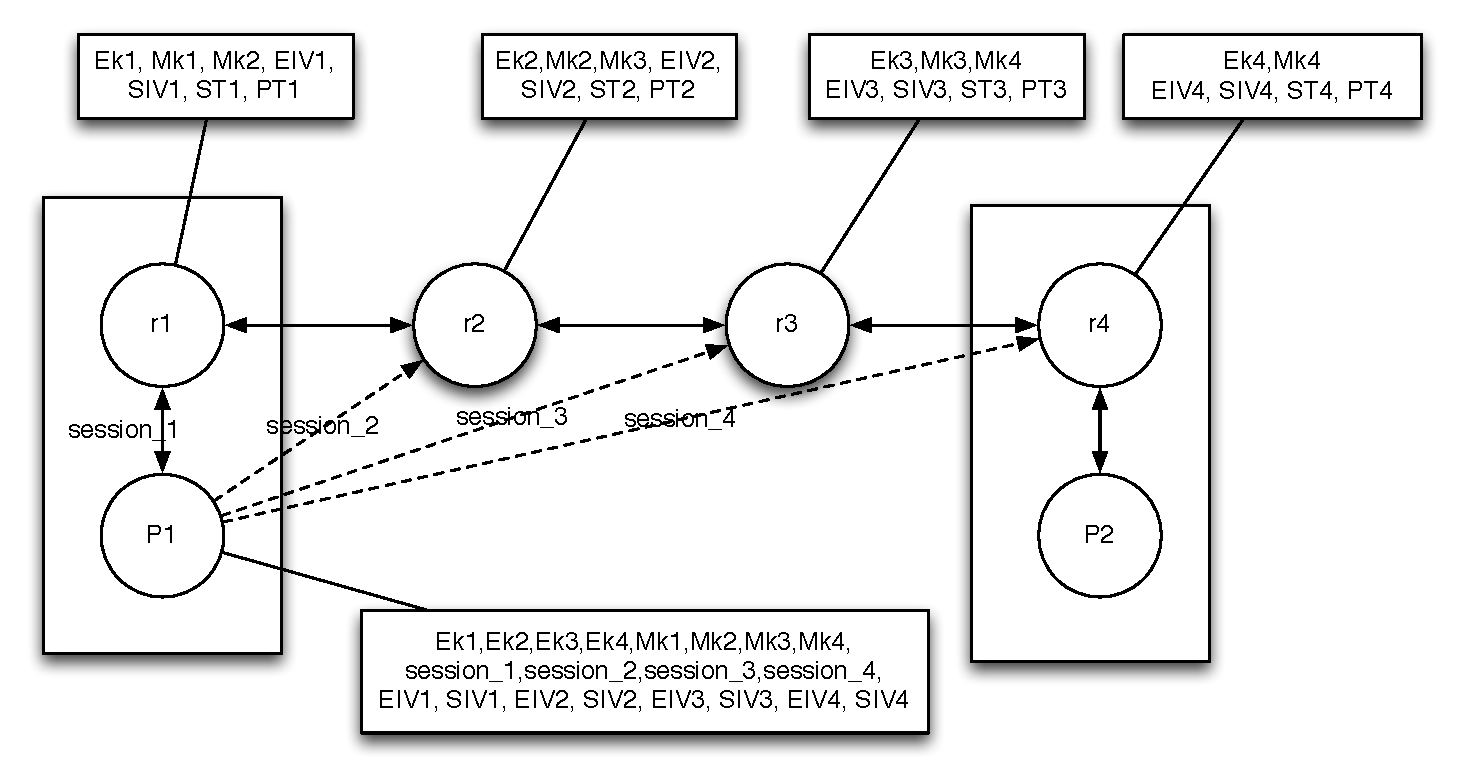
\includegraphics[scale=0.5]{./images/circuit.pdf}
\end{center}
\caption{Sample session-based circuit between a consumer $C$ and producer $P$ with ARs $r_1,r_2,r_3,r_4$, where the end routers on the path are run on the same node as $C$ and $P$.}
\label{fig:circuit}
\end{figure*}

\subsection{AND\=aNA-v2 Circuit Usage}

We note that anonymous routers must be chosen in a \emph{mutually excluse} manner, meaning that they do not change share the same name prefix or are from the same organization (see Figure \ref{fig:pool}). This requirement is needed for ensuring anonymity. After a circuit and the corresponding sessions have been created between the consumer and each anonymous router, usage of the circuit proceeds as per the original {\sf AND\=aNAv2} design. Specifically, there are three main operations that need to be defined: encrypted interest generation, AR interest forwarding, and AR content handling. In what we follows we present the details of each of these procedures as needed for {\sf AND\=aNA-v2}. We begin with the encrypted interest generation procedure (shown in Algorithm \ref{alg:enc_int_gen}) in which a consumer $C$ particpating in a particular \emph{application} session with a producer $P$ wraps an interest for the session to be sent into the anonymizing circuit. A wrapped (encrypted) interest from $r_i$ to $r_j$ ($i \leq j$) is denoted as $\overline{\mathsf{int}}_i^j$, meaning that the original plaintext interests $\mathsf{int}$ cannot be retrieve unless encrypted by each router $r_i,r_{i+1},\dots,r_j$, in that order. Thus, the original wrapped interest is denoted as $\overline{\mathsf{int}}_1^n$.

\begin{figure*}[ht!]
\begin{center}
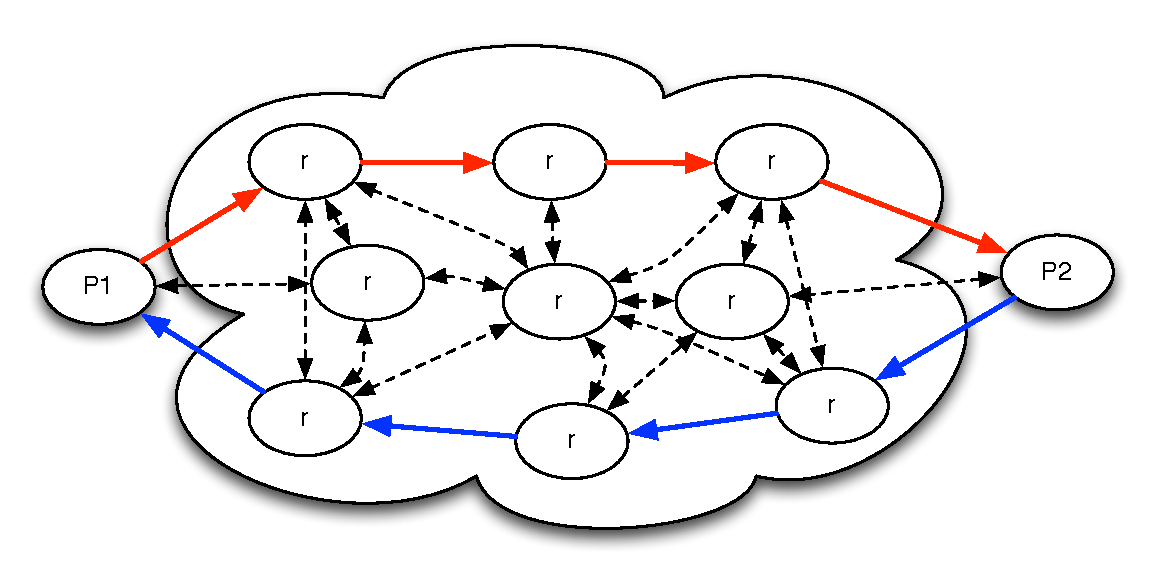
\includegraphics[scale=0.5]{./images/pool.pdf}
\end{center}
\caption{A sample bidirectional circuit configuration in which two parties communicate using mutually exclusive ARs in both directions. Note that it is not required for each circuit to be the same length, nor is it required that the intersection of the routers for each direction of the circuit to be empty (i.e., routers may \emph{unknowingly} support sessions traversing in both directions).}
\label{fig:pool}
\end{figure*}

\begin{algorithm}[ht!]
  \caption{Encrypted Interest Generation}
  \begin{algorithmic}[1]
    \Require{Interest $\mathsf{int}$, circuit length $n$, AR pool $\mathcal{R}$}
    \Ensure{Encrypted interest $\overline{\mathsf{int}}_{1}^{n}$}
\State $\overline{\mathsf{int}} = \mathsf{int}$
\For{$i = n$ \textbf{ downto } $1$}
  \State $\mathsf{SIndex}_i := H(\mathsf{session}_i + \mathsf{SIV}_i)$
  \State $\mathsf{SIV}_i = \mathsf{SIV}_i + 1$ (mod $2^{\kappa}$)
  \State $\overline{\mathsf{int}}_i^n = R_i / \mathsf{SIndex}_i / \mathsf{Encrypt}_{E_{k_i}}(\overline{\mathsf{int}}, \mathsf{timestamp})$
\EndFor
\State \Return $\overline{\mathsf{int}}_1^n$
\end{algorithmic}
\label{alg:enc_int_gen}
\end{algorithm}

\begin{algorithm}[ht!]
  \caption{AR Encrypted Interest Forwarding}
  \begin{algorithmic}[1]
    \Require{$\overline{\mathsf{int}}_i^j$}
    \Ensure{$(\overline{\mathsf{int}}_{i+1}^j, \mathsf{session}_i)$ or discarded packet}
\If{$\mathsf{SIndex}_i \in \mathsf{ST}_i$}
  \State Let $(\mathsf{session}_i, E_{k_i}, M_{k_i}, \mathsf{EIV}_i, \mathsf{SIV}_i)$ be the session information associated with $\mathsf{SIndex}_i$
  \State $\mathsf{SIV}_i := \mathsf{SIV}_i + 1$ (mod $2^{\kappa}$)
  \State $\mathsf{SIndex}_i := H(\mathsf{session}_i + \mathsf{SIV}_i)$
  \State Update $(\mathsf{SIndex}_i, \mathsf{session}_i, \mathsf{SIV}_i)$ in the session table $\mathsf{ST}_i$
  \State $(\overline{\mathsf{int}}_{i+1}^{j}, timestamp) := \mathsf{Decrypt}_{E_{k_i}}(\overline{\mathsf{int}}_{i}^{j})$
  \If{decryption fails or $\mathsf{timestamp}$ is not current}
    \State Discard $\overline{\mathsf{int}}_{i}^{j}$
  \Else
    \State Persist tuple $T_i = (\overline{\mathsf{int}}_{i}^{j}, \overline{\mathsf{int}}_{i+1}^{j}, \mathsf{session}_i)$ to pending interest table $\mathsf{PT}_i$
    \State \Return $(\overline{\mathsf{int}}_{i+1}^{j}, \mathsf{session}_i)$
  \EndIf
\Else
  \State Discard $\overline{\mathsf{int}}_{i}^{j}$ \Comment{Some form of interest flooding prevention should be employed here}
\EndIf
\end{algorithmic}
\label{alg:enc_int_forward}
\end{algorithm}

\begin{algorithm}[ht!]
  \caption{AR Content Handling}
  \begin{algorithmic}[1]
    \Require{Content $\overline{data_{i+1}^j}$ in response to interest $\overline{\mathsf{int}}_{i+1}^{j}$}
    \Ensure{Encrypted data packet $data_{i}^j$}
\State Recover tuple $T_i = (\overline{\mathsf{int}}_{i}^{j}, \overline{\mathsf{int}}_{i+1}^{j}, \mathsf{session}_i)$ based on $data_{i+1}^j$
\State Parse $\overline{data_{i+1}^j}$ as a tuple $(data_{i+1}^j, \sigma_{i+1})$
\If{$\sigma_{i+1} = \epsilon$ and $M_{k_{i+1}} = \epsilon$} \Comment{Last hop router - does not verify MAC}
  \State Pass
\ElsIf{$\sigma_{i+1} \not= \epsilon$ and $M_{k_{i+1}} \not= \epsilon$}
  \If{$\sigma_{i+1} = \mathsf{Verify}_{M_{k_{i+1}}}(data_{i+1}^j)$}
    \State Pass
  \Else
    \State \Return $\mathsf{Error}$ \Comment{MAC verification did not pass}
  \EndIf
\Else \Comment{There was either a tag or we don't have the upstream MAC key - either way, we error}
  \State \Return $\mathsf{Error}$
\EndIf

\State Remove signature and name from $data_{i+1}^j$    
\State Create new empty data packet $data_i^j$
\State Set name on $data_i^j$ as the name on $\overline{\mathsf{int}}_{i}^{j}$
\State $data_i^j := \mathsf{Encrypt}_{E_{k_i}}(data_i^j)$
\State $\sigma_i := \mathsf{MAC}(data_i^j)$
\State $\overline{data_{i}^j} = ((data_i^j, \sigma_i))$
\State \Return $\overline{data_{i}^j}$

\end{algorithmic}
\label{alg:ar_content_handler}
\end{algorithm}

\begin{figure*}[ht!]
\begin{center}
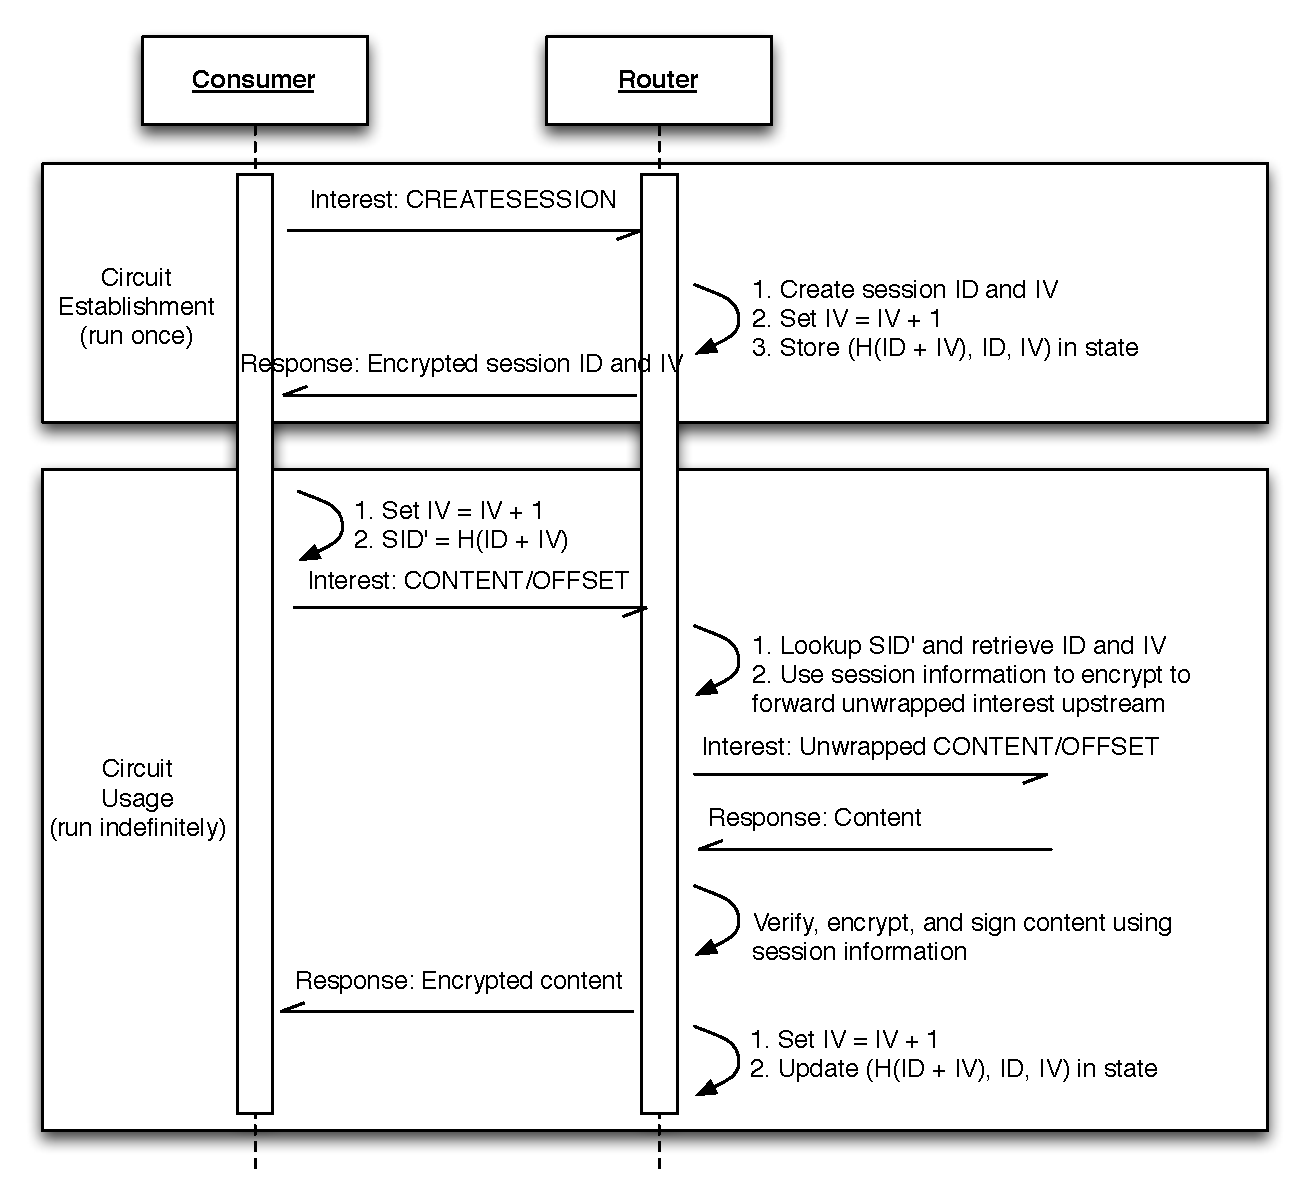
\includegraphics[scale=0.65]{./images/circuit_usage.pdf}
\end{center}
\caption{Visual depiction of the interaction between the consumer and the first hop router. The procedure repeats in the same manner for all further upstream routers after each interest is unrolled and resulting content is encrypted.}
\label{fig:circuit_usage}
\end{figure*}
